
\chapter{Random Variables}

\section{Important/Useful Theorems}

\subsection{Chebyshev's Inequality}

\begin{equation}
	P \{ |\xi| > \epsilon \} \leq \frac{1}{\epsilon^2} \textbf{E}\xi^2
\end{equation}


\section{Answers to Problems}

\subsection{}
%problem 4.1
Thinking of this problem as 4 buckets each with 2 possibilities paves a clear way to the solution of the problem.  There are $2^4 = 16$ possibilities.  There is only one way for them to all be green ($\xi = 4$), and again only one way for 3 greens followed by one red ($\xi = 3$).  Once you have get to $\xi = 2$, then the last light can be either green or red giving two possibilities then at $\xi = 1$ you have two lights that can be either red or green giving 4 possibilities.  Clearly, then, there are 8 for the case of $\xi = 0$.  

\begin{equation}
	P(\xi) = \left\{ \begin{array}{rl}
	\frac{1}{2}, \xi=0  \\
	\frac{1}{4}, \xi=1  \\
	\frac{1}{8}, \xi=2  \\
	\frac{1}{16}, \xi=3  \\
	\frac{1}{16}, \xi=4
       \end{array} \right.
\label{answer4.1}
\end{equation}
\textbf{Answer not verified}

\subsection{}
%problem 4.2
To summarize what we want here:
\begin{eqnarray}
	\xi_1 \neq \xi_2 \\
	\Phi_{\xi_1}(x) = \Phi_{\xi_2}(x) \\
	\int_{-\infty}^x p_{\xi_1}(x')dx' = \int_{-\infty}^x p_{\xi_2}(x')dx'
\end{eqnarray}
Since the question does not rule out the possibility that the probability distributions are the same, we can just say that $\xi_1$ is the outcome of a coin-flip experiment and that $\xi_2$ is the outcome of the first spin measurement of an EPR experiment. 
\textbf{Answer not verified}

\subsection{}
%problem 4.3
If 
\begin{equation}
	p(x)dx = \frac{dx}{b-a}
\end{equation}
then
\begin{equation}
	\Phi(x) = \int_{-a}^x p(x')dx' = \int_{a}^x \frac{dx'}{b-a}
\end{equation}
\begin{equation}
	\Phi(x) = \frac{x - a}{b-a}
\label{answer4.3}
\end{equation}
\textbf{Answer not verified}

\subsection{}
%problem 4.4
The distribution is clearly not normalized so the first step will be to normalise it.

\begin{equation}
	\int^{\infty}_{-\infty} \frac{a}{x^2+1}dx = 1 = a \pi
\end{equation}

\begin{equation}
	a = \frac{1}{\pi}
\label{answer4.4a}
\end{equation}

Just by definition:
\begin{equation}
	\Phi(x) = \int^{x}_{\infty} \frac{1}{\pi(x'^2+1)}dx' = \left \frac{\arctan x'}{\pi} \right] ^x_{-\infty} = \frac{\arctan x}{\pi}+\frac{1}{2}
\label{answer4.4b}
\end{equation}
and last but not least:
\begin{equation}
	P( \{ -1 \leq x \leq 1 \} = \int^{1}_{-1} \frac{1}{\pi(x'^2+1)}dx' = \frac{1}{2}
\label{answer4.4c}
\end{equation}

\textbf{Answers verified}

\subsection{}
%problem 4.5
Once again we start by normalizing
\begin{equation}
	1= \int^{\infty}_{0} a x^2 e^{-k x} dx = -\left \frac{e^{-k x} \left(2+2 k x+k^2 x^2\right)}{k^3} \right]^{\infty}_{0}= \frac{2 a}{k^3}
	\end{equation}
\begin{equation}
	a = \frac{k^3}{2}
\label{answer4.5a}
\end{equation}
\begin{equation}
	\Phi(x) = \int^{x}_{0} \frac{k^3}{2}x'^2 e^{-k x'}dx' = 1 - \frac{e^{-k x} \left(2+2 k x+k^2 x^2\right)}{2}
\label{answer4.5b}
\end{equation}
\begin{equation}
	P( \{ 0 \leq x \leq \frac{1}{k} \} = \int_{0}^{\frac{1}{k}} \frac{k^3}{2}x^2 e^{-k x}dx = \frac{2e - 5}{2 e}
\label{answer4.4c}
\end{equation}
\textbf{Answer not verified}



\subsection{}
%problem 4.6
\begin{equation}
	\Phi(\infty) = 1 \Rightarrow 1 = a + \frac{b \pi}{2}
\end{equation}
\begin{equation}
	\Phi(-\infty) = 0 \Rightarrow 0 = a - \frac{b \pi}{2}
\end{equation}
Which you can solve to get
\begin{eqnarray}
	b = \frac{1}{\pi} \\
	a = \frac{1}{2}
\end{eqnarray}
Since $\Phi$ is the integral of $p$, we can take the derivative of it and then make sure it's normalized.
\begin{equation}
	p(x) = \frac{d \Phi}{dx} = \frac{1}{2 \pi \left(1+\frac{x^2}{4}\right)}
\end{equation}
And the normalization is indeed still correct!

\textbf{Answer not verified}

\subsection{}
%problem 4.6
The area of the table is simply $\pi R^2$ and the are of each of the smaller circles are $\pi r^2$.  The ratio of the sum of the area of the two circles to the total table area will be the chance that one of the circles gets hit: $p = \frac{2r^2}{R^2}$.
\textbf{Answer verified}


\subsection{}
%problem 4.7
Just like in example 2 in the book, this problem will go by very well if we draw a picture indicating the given criteria:

\begin{figure}[hbtp]
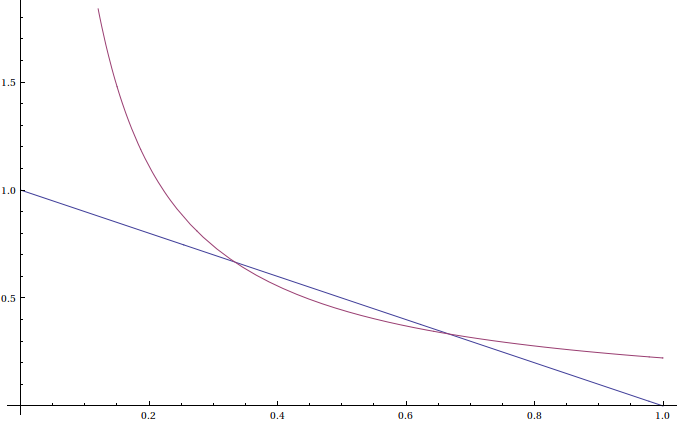
\includegraphics[width=\textwidth]{overlap.png}
\caption{The Desired Region}
\end{figure}
Where does this come from?
\begin{eqnarray}
	x_1 + x_2 \leq 1 \\ 
	x_2 \leq 1 - x_1
\end{eqnarray}
which is the straight line.
\begin{eqnarray}
	x_1x_2 \leq \frac{2}{9} \\ 
	x_2 \leq \frac{2}{9 x_1}
\end{eqnarray}
A little bit of algebra shows that these two lines intersect at $\frac{1}{3}$ and $\frac{2}{3}$ so the area underneath the straight line but not above the curved line is
\begin{eqnarray}
	A =\int_0^{\frac{1}{3}}(1-x)dx + \int_{\frac{1}{3}}^{\frac{2}{3}}\frac{2}{9x}dx + \int_{\frac{2}{3}}^{1}(1-x)dx \\ 
	= \frac{5}{18} + \int_{\frac{1}{3}}^{\frac{2}{3}}\frac{2}{9x}dx + \frac{1}{18} \\
	= \frac{1}{3} + \int_{\frac{1}{3}}^{\frac{2}{3}}\frac{2}{9x}dx \\ 
	= \frac{1}{3	} + \frac{2 \ln 2}{9} \approx 0.487366
\end{eqnarray}
And the answer is properly normalized since the initial probability distributions were unity (the box length is only 1).
\textbf{Answer  verified}


\subsection{}
%problem 4.9
As we showed in example number 4, $p_{\eta}$ is the convolution of $p_{\xi_1}$ and $p_{\xi_2}$.
\begin{eqnarray}
	p_{\eta}(y) = \int_{-\infty}^{\infty} p_{\xi_1}(y-x)p_{\xi_2}(x)dx
\end{eqnarray}
I think the integration will look more logical if we stick in Heaviside step-functions.
\begin{eqnarray}
	p_{\eta}(y) = \frac{1}{6} \int_{-\infty}^{\infty}e^{-\frac{y-x}{3}}e^{-\frac{x}{3}}H(y-x)H(x)dx
\end{eqnarray}
Clearly $x$ has to be greater than zero and $y$ must be greater than x, leading to the following limits of integration.
\begin{eqnarray}
	p_{\eta}(y) = \frac{1}{6} \int_{0}^{y}e^{-\frac{y-x}{3}}e^{-\frac{x}{3}}dx \\
	= e^{-\frac{y}{3}}\left(1- e^{-\frac{y}{6}}  \right)
\end{eqnarray}
Only when y is greater than zero!
\textbf{Answer verified}

\subsection{}
%problem 4.10
Due to the magic of addition, finding the probability distribution of $\xi_1 + \xi_2 + \xi_3$ is no different than the probability distribution of $(\xi_1 + \xi_2) + \xi_3$ but we already know what the probability distribtution of the parenthesized quantity is:
\begin{equation}
	p_{\xi_1 + \xi_2}(y) = \int_{-\infty}^{\infty} p_{\xi_1}(y-x)p_{\xi_2}(x)dx
\end{equation}
Therefore the total combination is
\begin{equation}
	p_{\xi_1 + \xi_2+ \xi_3}(z) = \int_{-\infty}^{\infty} p_{\xi_1 + \xi_2}(z-y)p_{\xi_3}(y)dx
\end{equation}
\begin{equation}
	p_{\xi_1 + \xi_2+ \xi_3}(z) = \int_{-\infty}^{\infty} \left[ \int_{-\infty}^{\infty} p_{\xi_1}(z-y-x)p_{\xi_2}(x)dx \right]p_{\xi_3}(y)dy
\end{equation}
\begin{equation}
	p_{\xi_1 + \xi_2+ \xi_3}(z) = \int_{-\infty}^{\infty}  \int_{-\infty}^{\infty} p_{\xi_1}(z-y-x)p_{\xi_2}(x)p_{\xi_3}(y)dx dy
\end{equation}
which is just a triple convolution.

\textbf{Answer not verified}

\subsection{}
%problem 4.11
\begin{equation}
	p_{\xi}(n) = \frac{1}{3^n}
\end{equation}
therefore
\begin{equation}
	\textbf{E}\xi = \sum_{n=1}^{\infty}\frac{n}{3^n} =  \frac{3}{4}
\label{answer4.11}
\end{equation}
\textbf{Answer not verified}

\subsection{}
%problem 4.12
Since finding a ball in one urn versus the other urn has nothing to do with each other, the events are clearly independent so we can multiply probabilities.  The probability of finding a white ball at any given urn is
\begin{equation}
	p_w = \frac{w}{w+b}
\end{equation}
If you find a white ball on the $n^{th}$ try then that means you found $n-1$ black balls before you got to the white ball.  
\begin{equation}
	p_w(n) = \frac{b^{n-1} w}{(w+b)^n}
\end{equation}
\begin{equation}
	\textbf{E}n = \sum_{i=1}^{\infty}n p_w(n) = \sum_{i=1}^{\infty}n \frac{b^{n-1} w}{(w+b)^n} = \frac{b+w}{w}
\end{equation}
Which is the total number of balls drawn, subtract one to get the average number of black balls drawn:
\begin{equation}
	m=\frac{b}{w}
\end{equation}
Now for the variance. to start with we need the average of the square of the random variable.
\begin{equation}
	\textbf{E}n^2 = \sum_{i=1}^{\infty}n^2 p_w(n) = \sum_{i=1}^{\infty}n^2 \frac{b^{n-1} w}{(w+b)^n} = \frac{(b+w) (2 b+w)}{w^2}
\end{equation}
\begin{equation}
	\textbf{D}n = \textbf{E}n^2 - (\textbf{E}n)^2 =  \frac{(b+w) (2 b+w)}{w^2} - \left( \frac{b+w}{w} \right)^2 = \frac{b^2+wb}{w^2}
\end{equation}
A note that we don't need to subtract anything for the variance since shifting a distribution over does not affect its variance: just its average.
\textbf{Answer verified}



\subsection{}
%problem 4.13
\begin{equation}
	\textbf{E}\xi = \int_{-\infty}^{\infty} x\frac{1}{2}e^{-|x|} = 0
\end{equation}
because the function is even about $x=0$.
\begin{equation}
	\textbf{E}\xi^2 = \int_{-\infty}^{\infty} x^2\frac{1}{2}e^{-|x|} = 2
\end{equation}
Therefore:
\begin{equation}
	\textbf{D}\xi = \textbf{E}\xi^2 - (\textbf{E}\xi)^2 = 2
\end{equation}
\textbf{Answer verified}




\subsection{}
%problem 4.14
\begin{equation}
	\textbf{E}x = \int_{a-b}^{a+b} \frac{xdx}{2b} = a	
\end{equation}
\begin{equation}
	\textbf{E}x^2 = \int_{a-b}^{a+b} \frac{x^2dx}{2b} = a^2+\frac{b^2}{3}
\end{equation}
Therefore:
\begin{equation}
	\textbf{D}x = \frac{b^2}{3}
\end{equation}
\textbf{Answer verified}


\subsection{}
%problem 4.15
If the distribution function is 
\begin{equation}
	\Phi_{\xi}(x) = a + b \arcsin x, |x| \leq 1
\end{equation}
then it must fulfill the proper boundary conditions as specified by both the problem and the definition of a distribution function.
\begin{equation}
	\Phi_{\xi}(-1)= 0 = a - b \frac{\pi}{2}
\end{equation}
\begin{equation}
	\Phi_{\xi}(1) = 1 = a + b \frac{\pi}{2}
\end{equation}
Some easy algebra gets you
\begin{eqnarray}
	\Phi_{\xi}(x) = \frac{1}{2} + \frac{1}{\pi} \arcsin x
\end{eqnarray}
Therefore:
\begin{equation}
	p_{\xi}(x) = \frac{1}{\pi\sqrt{1-x^2}}
\end{equation}
\begin{eqnarray}
	\textbf{E}x = \int_{-1}^{1} \frac{x dx}{\pi\sqrt{1-x^2}} = 0 \\
	\textbf{D}x = \int_{-1}^{1} \frac{x^2 dx}{\pi\sqrt{1-x^2}} = \frac{1}{2}
\end{eqnarray}
\textbf{Answer verified}



\subsection{}
%problem 4.16
Each side of the die has the same probability, $\frac{1}{6}$
\begin{equation}
	\textbf{E}x = \sum_{i=1}^6 \frac{i}{6} = \frac{7}{2}
\end{equation}
\begin{equation}
	\textbf{E}x^2 = \sum_{i=1}^6 \frac{i^2}{6} = \frac{91}{6}
\end{equation}
Therefore:
\begin{equation}
	\textbf{D}x = \frac{91}{6} - \left( \frac{7}{2} \right)^2 = \frac{91}{6} - \frac{49}{4} = \frac{35}{12}
\end{equation}
\textbf{Answer verified}

\subsection{}
%problem 4.17
This problem may seem difficult until you realize that being $\pm \frac{5}{2}$ away from the mean means you're at either 1 or 6, meaning that there's a unity probability of being that far from the mean.  Chebyshev's inequality, however, would have us believe that 
\begin{equation}
	P \{ |x + \textbf{E}x| > \frac{5}{2}  \} \leq \frac{4}{25} \frac{91}{6} = \frac{182}{75} = 2.42667
\end{equation}
which is not only far off from the actual answer, it's also unphysical to have probabilities greater than 1!
\textbf{Answer not verified}

\subsection{}
%problem 4.18
We want to consider the probability distribution of $\xi$ by way of $\eta$
\begin{equation}
	\eta = e^{\frac{a\xi}{2}} 
\end{equation}
We know from Chebyshev's identity:

\begin{equation}
	P\{ \eta > \epsilon(\eta) \} \leq \frac{\textbf{E}\eta^2}{\epsilon(\eta)^2} 
\end{equation}
Let $\epsilon$ be the error in $\xi$ we're looking for.
\begin{equation}
	P\{ \xi > \epsilon \} \leq \frac{\textbf{E}(e^{\frac{a\xi}{2}})^2}{(e^{\frac{a\epsilon}{2}})^2} 
\end{equation}
\begin{equation}
	P\{ \xi > \epsilon \} \leq \frac{\textbf{E}e^{a\xi}}{e^{a\epsilon}} 
\end{equation}
\textbf{Answer not verified}


\subsection{}
%problem 4.19
First some initial calculations:
\begin{eqnarray}
	\textbf{E}\xi = \frac{1}{4} \left( -2+-1+1+2  \right) = 0 \\
	\textbf{E}\xi^2 = \frac{1}{4} \left( (-2)^2+(-1)^2+1^2+2^2  \right) = \frac{10}{4} = \frac{5}{2} = \textbf{E}\eta \\
	\textbf{E}\xi^4 = \frac{1}{4} \left( (-2)^4+(-1)^4+1^4+2^4  \right) = \frac{34}{4} = \frac{17}{2} = \textbf{E}\eta^2
\end{eqnarray}
Now, we know that
\begin{eqnarray}
	r = \frac{\textbf{E} \left[ (\xi - \textbf{E}\xi)(\eta - \textbf{E}\eta)  \right]}{(\textbf{E}\xi^2 - (\textbf{E}\xi)^2)(\textbf{E}\eta^2 - (\textbf{E}\eta)^2)}
\end{eqnarray}
The denominator $D$ is the easiest:
\begin{equation}
	D = \left( \frac{5}{2} - 0 \right)\left( \frac{17}{2} - \frac{5^2}{2^2} \right) = \frac{45}{8}
\end{equation}
Now for the numerator:
\begin{eqnarray}
	\textbf{E} \left[ (\xi - \textbf{E}\xi)(\eta - \textbf{E}\eta)  \right] \\
	= \frac{1}{16} \left[  \sum_{\xi, \eta} (\xi - \textbf{E}\xi)(\eta - \textbf{E}\eta)      \right]
\end{eqnarray}
If we look at the set we'll be summing over, we have ${\xi - \textbf{E}\xi} = -2, -1, 1, 2$ and ${\eta - \textbf{E}\eta} = \frac{3}{2}, -\frac{3}{2}, -\frac{3}{2}, \frac{3}{2}$ and clearly, since we have to sum over all possible products, since both distributions are symmetric about 0, the sum will go to zero.
\begin{equation}
	r=0
\end{equation}
\textbf{Answer not verified}

\subsection{}
%problem 4.20
First some initial calculations:
\begin{eqnarray}
	\textbf{E}x_1 = \int_0^{\frac{\pi}{2}} x_1 \sin x_1 \sin x_2 dx_1dx_2 = 1 \\
	\textbf{E}x_2 = 1 \\
	\textbf{E}x_1^2 = \int_0^{\frac{\pi}{2}} x_1^2 \sin x_1 \sin x_2 dx_1dx_2 = (\pi - 2) \\
	\textbf{E}x_2^2 = (\pi - 2) \\
\end{eqnarray}
\begin{eqnarray}
	\textbf{E} \left[ (x_1 - \textbf{E}x_1)(x_2 - \textbf{E}x_2)  \right] \\
	= \int_0^{\frac{\pi}{2}} \int_0^{\frac{\pi}{2}} \left[(x_1 - 1)(x_2 - 1)\right]\sin x_1 \sin x_2 dx_1dx_2 = 0 \\
	\sigma_1 \sigma_2 =  \sqrt{(\pi - 2)- 1}\sqrt{(\pi - 2) - 1} = (\pi - 3) \\
	r= \frac{0}{(\pi - 3)} = 0
\end{eqnarray}
\textbf{Answer not verified}

\subsection{}
%problem 4.21
First some initial calculations:
\begin{eqnarray}
	\textbf{E}x_1 = \frac{1}{2}\int_0^{\frac{\pi}{2}} x_1 \sin (x_1 + x_2) dx_1dx_2 = \frac{\pi}{4} \\
	\textbf{E}x_2 = \frac{\pi}{4} \\
	\textbf{E}x_1^2 = \frac{1}{2}\int_0^{\frac{\pi}{2}} x_1^2 \sin (x_1 + x_2) dx_1dx_2 = -2+\frac{\pi}{2} +\frac{\pi ^2}{8} \\
	\textbf{E}x_2^2 = -2+\frac{\pi}{2} +\frac{\pi ^2}{8} \\
\end{eqnarray}
\begin{eqnarray}
	\textbf{E} \left[ (x_1 - \textbf{E}x_1)(x_2 - \textbf{E}x_2)  \right] \\
	= \frac{1}{2}\int_0^{\frac{\pi}{2}} \int_0^{\frac{\pi}{2}} \sin (x_1 + x_2) \left[(x_1 - \frac{\pi}{2})(x_2 - \frac{\pi}{2})\right]dx_1dx_2  = -\frac{1}{16} (\pi -4)^2 \\
	\sigma_1\sigma_2 = -2+\pi +\frac{\pi ^2}{2} +\frac{\pi^2}{8} - \frac{\pi^2}{16} = -2+\pi +\frac{\pi ^2}{2} +\frac{\pi^2}{16} \\
	r = \frac{-\frac{1}{16} (\pi -4)^2}{-2+\pi +\frac{\pi ^2}{2} +\frac{\pi^2}{16}}
\end{eqnarray}
\textbf{Answer verified}

\subsection{}
%problem 4.22
Ill-defined problem, don't feel like translating: \textbf{SKIPPED}

\subsection{}
%problem 4.23
Based off 4.22: \textbf{SKIPPED}

\subsection{}
%problem 4.21
\begin{eqnarray}
	E\xi = \int_{-\infty}^{\infty} \frac{x}{\pi(1+x^2)}dx = \left \frac{\log \left(x^2+1\right)}{2 \pi } \right]_{-\infty}^{\infty} \rightarrow \infty \\
	E\xi^2 = \int_{-\infty}^{\infty} \frac{x^2}{\pi(1+x^2)}dx = \left \frac{x}{\pi }-\frac{\tan ^{-1}(x)}{\pi } \right]_{-\infty}^{\infty} \rightarrow \infty
\end{eqnarray}
Neither integral actually converges so we cannot define averages or dispersions for this distribution.
\textbf{Answer verified}
%%answer template
%\subsection{}
%%problem n.n
%
%
%\begin{equation}
%	
%\label{answern.n}
%\end{equation}
%\textbf{Answer [not] verified}





